\documentclass[]{article}
\usepackage{lmodern}
\usepackage{amssymb,amsmath}
\usepackage{ifxetex,ifluatex}
\usepackage{fixltx2e} % provides \textsubscript
\ifnum 0\ifxetex 1\fi\ifluatex 1\fi=0 % if pdftex
  \usepackage[T1]{fontenc}
  \usepackage[utf8]{inputenc}
\else % if luatex or xelatex
  \ifxetex
    \usepackage{mathspec}
  \else
    \usepackage{fontspec}
  \fi
  \defaultfontfeatures{Ligatures=TeX,Scale=MatchLowercase}
\fi
% use upquote if available, for straight quotes in verbatim environments
\IfFileExists{upquote.sty}{\usepackage{upquote}}{}
% use microtype if available
\IfFileExists{microtype.sty}{%
\usepackage{microtype}
\UseMicrotypeSet[protrusion]{basicmath} % disable protrusion for tt fonts
}{}
\usepackage[margin=1in]{geometry}
\usepackage{hyperref}
\hypersetup{unicode=true,
            pdftitle={Facial Keypoint Detection - Documentation},
            pdfauthor={Henry Perschk, Lucas Stegger},
            pdfborder={0 0 0},
            breaklinks=true}
\urlstyle{same}  % don't use monospace font for urls
\usepackage{color}
\usepackage{fancyvrb}
\newcommand{\VerbBar}{|}
\newcommand{\VERB}{\Verb[commandchars=\\\{\}]}
\DefineVerbatimEnvironment{Highlighting}{Verbatim}{commandchars=\\\{\}}
% Add ',fontsize=\small' for more characters per line
\usepackage{framed}
\definecolor{shadecolor}{RGB}{248,248,248}
\newenvironment{Shaded}{\begin{snugshade}}{\end{snugshade}}
\newcommand{\KeywordTok}[1]{\textcolor[rgb]{0.13,0.29,0.53}{\textbf{{#1}}}}
\newcommand{\DataTypeTok}[1]{\textcolor[rgb]{0.13,0.29,0.53}{{#1}}}
\newcommand{\DecValTok}[1]{\textcolor[rgb]{0.00,0.00,0.81}{{#1}}}
\newcommand{\BaseNTok}[1]{\textcolor[rgb]{0.00,0.00,0.81}{{#1}}}
\newcommand{\FloatTok}[1]{\textcolor[rgb]{0.00,0.00,0.81}{{#1}}}
\newcommand{\ConstantTok}[1]{\textcolor[rgb]{0.00,0.00,0.00}{{#1}}}
\newcommand{\CharTok}[1]{\textcolor[rgb]{0.31,0.60,0.02}{{#1}}}
\newcommand{\SpecialCharTok}[1]{\textcolor[rgb]{0.00,0.00,0.00}{{#1}}}
\newcommand{\StringTok}[1]{\textcolor[rgb]{0.31,0.60,0.02}{{#1}}}
\newcommand{\VerbatimStringTok}[1]{\textcolor[rgb]{0.31,0.60,0.02}{{#1}}}
\newcommand{\SpecialStringTok}[1]{\textcolor[rgb]{0.31,0.60,0.02}{{#1}}}
\newcommand{\ImportTok}[1]{{#1}}
\newcommand{\CommentTok}[1]{\textcolor[rgb]{0.56,0.35,0.01}{\textit{{#1}}}}
\newcommand{\DocumentationTok}[1]{\textcolor[rgb]{0.56,0.35,0.01}{\textbf{\textit{{#1}}}}}
\newcommand{\AnnotationTok}[1]{\textcolor[rgb]{0.56,0.35,0.01}{\textbf{\textit{{#1}}}}}
\newcommand{\CommentVarTok}[1]{\textcolor[rgb]{0.56,0.35,0.01}{\textbf{\textit{{#1}}}}}
\newcommand{\OtherTok}[1]{\textcolor[rgb]{0.56,0.35,0.01}{{#1}}}
\newcommand{\FunctionTok}[1]{\textcolor[rgb]{0.00,0.00,0.00}{{#1}}}
\newcommand{\VariableTok}[1]{\textcolor[rgb]{0.00,0.00,0.00}{{#1}}}
\newcommand{\ControlFlowTok}[1]{\textcolor[rgb]{0.13,0.29,0.53}{\textbf{{#1}}}}
\newcommand{\OperatorTok}[1]{\textcolor[rgb]{0.81,0.36,0.00}{\textbf{{#1}}}}
\newcommand{\BuiltInTok}[1]{{#1}}
\newcommand{\ExtensionTok}[1]{{#1}}
\newcommand{\PreprocessorTok}[1]{\textcolor[rgb]{0.56,0.35,0.01}{\textit{{#1}}}}
\newcommand{\AttributeTok}[1]{\textcolor[rgb]{0.77,0.63,0.00}{{#1}}}
\newcommand{\RegionMarkerTok}[1]{{#1}}
\newcommand{\InformationTok}[1]{\textcolor[rgb]{0.56,0.35,0.01}{\textbf{\textit{{#1}}}}}
\newcommand{\WarningTok}[1]{\textcolor[rgb]{0.56,0.35,0.01}{\textbf{\textit{{#1}}}}}
\newcommand{\AlertTok}[1]{\textcolor[rgb]{0.94,0.16,0.16}{{#1}}}
\newcommand{\ErrorTok}[1]{\textcolor[rgb]{0.64,0.00,0.00}{\textbf{{#1}}}}
\newcommand{\NormalTok}[1]{{#1}}
\usepackage{graphicx,grffile}
\makeatletter
\def\maxwidth{\ifdim\Gin@nat@width>\linewidth\linewidth\else\Gin@nat@width\fi}
\def\maxheight{\ifdim\Gin@nat@height>\textheight\textheight\else\Gin@nat@height\fi}
\makeatother
% Scale images if necessary, so that they will not overflow the page
% margins by default, and it is still possible to overwrite the defaults
% using explicit options in \includegraphics[width, height, ...]{}
\setkeys{Gin}{width=\maxwidth,height=\maxheight,keepaspectratio}
\IfFileExists{parskip.sty}{%
\usepackage{parskip}
}{% else
\setlength{\parindent}{0pt}
\setlength{\parskip}{6pt plus 2pt minus 1pt}
}
\setlength{\emergencystretch}{3em}  % prevent overfull lines
\providecommand{\tightlist}{%
  \setlength{\itemsep}{0pt}\setlength{\parskip}{0pt}}
\setcounter{secnumdepth}{5}
% Redefines (sub)paragraphs to behave more like sections
\ifx\paragraph\undefined\else
\let\oldparagraph\paragraph
\renewcommand{\paragraph}[1]{\oldparagraph{#1}\mbox{}}
\fi
\ifx\subparagraph\undefined\else
\let\oldsubparagraph\subparagraph
\renewcommand{\subparagraph}[1]{\oldsubparagraph{#1}\mbox{}}
\fi

%%% Use protect on footnotes to avoid problems with footnotes in titles
\let\rmarkdownfootnote\footnote%
\def\footnote{\protect\rmarkdownfootnote}

%%% Change title format to be more compact
\usepackage{titling}

% Create subtitle command for use in maketitle
\newcommand{\subtitle}[1]{
  \posttitle{
    \begin{center}\large#1\end{center}
    }
}

\setlength{\droptitle}{-2em}
  \title{Facial Keypoint Detection - Documentation}
  \pretitle{\vspace{\droptitle}\centering\huge}
  \posttitle{\par}
  \author{Henry Perschk, Lucas Stegger}
  \preauthor{\centering\large\emph}
  \postauthor{\par}
  \predate{\centering\large\emph}
  \postdate{\par}
  \date{7 1 2017}


\begin{document}
\maketitle

{
\setcounter{tocdepth}{2}
\tableofcontents
}
\section{Introduction}\label{introduction}

The fkdR (short for Facial Keypoints Detection in R) package is intended
for predicting facial keypoint positions like the centers of the eyes or
the nose tip for example. It furthermore provides functionality to train
models for facial keypoint recognition. This is achieved by using the
mlR package to make use of a standardized interface for e.g.~resampling
or tuning. As of now we implemented a patch search learner with mlR to
show the concept of our package and the way image data is handled. Our
research showed, that best results for image recognition by
machine-learning are achieved by Deep Neural Nets. Thus, we moreover
composed first a multi-layer-perceptron as well as a convolutional
neural net, both based on tensorflow. The data we use in this package is
based on the
\href{https://www.kaggle.com/c/facial-keypoints-detection}{Facial
Keypoints Detection contest} posted on Kaggle.

\begin{itemize}
\tightlist
\item
  structure of package?
\item
  structure of documentation
\end{itemize}

\section{Loading and Preprocessing the
Data}\label{loading-and-preprocessing-the-data}

The datasets are provided by the authors of the Kaggle contest as two
csv files. The training data consists of 7049 images, whereas the test
data consists of 1783 images. The images are 96x96 pixel grayscaled
images stored as column-wise vector of length 9216. Having a look at the
keypoints in the training dataset we found out that it actually is
composed of two differen training datasets, one with 4 keypoints and the
other with 15 keypoints (also containing the 4 of the other dataset).
These 4 keypoints are:

\begin{itemize}
\tightlist
\item
  left eye center
\item
  right eye center
\item
  nose tip
\item
  nose tip
\end{itemize}

The remaining keypoints are the following:

\begin{itemize}
\item
  left eye inner corner
\item
  left eye outer corner
\item
  right eye inner corner
\item
  right eye outer corner
\item
  left eyebrow inner end
\item
  left eyebrow outer end
\item
  right eyebrow inner end
\item
  right eyebrow outer end
\item
  mouth left corner
\item
  mouth right corner
\item
  mouth center bottom lip
\item
  histogram equalization
\item
  transformation in 1-dimensional data
\end{itemize}

\section{Patch Search Learner}\label{patch-search-learner}

The patch search learner we implemented is based on the
\href{https://www.kaggle.com/c/facial-keypoints-detection/details/getting-started-with-r}{Getting
Started Tutorial} from the
\href{https://www.kaggle.com/c/facial-keypoints-detection}{Facial
Keypoints Detection contest}. We used the logic and realized it using
\texttt{mlR}, which allowed us to make use of \texttt{mlR}'s
standardized interface for machine learning. Thus, we tried to improve
the results by making use of tuning and resampling. As usual the patch
search algorithm can be devided into training and prediction.

The basic idea behind the patch search learner is to extract all pixels
with a specific radius around each keypoint in each image. The extracted
pixels are refered to as patch. Afterwards, for each keypoint the mean
patch is calculated by calculating the mean of each pixel. This mean
patch can in a next step be used on any image containing the keypoint
(assuming it is also a 96x96 pixel grayscale image, where the face
ideally covers the whole width and height of the image and is
horizontally aligned). Predicting the keypoint is achieved by running
through the desired image pixel by pixel and again extracting the the
patch around this pixel. The point, where the extracted patch best
matches the trained mean patch is used as prediction.

\subsection{Training a Patch for a Facial
Keypoint}\label{patch-search-train}

As indicated the first step is to extract the patch for each keypoint
from each training image. One limitation using mlR was, that mlR as of
now does not offer an interface for regression with more than one
targets. This becomes a problem, as we are trying to train and predict
15 keypoints which consist of two coordinates. As explained in section
2, we solved the problem of predicting two coordinates by transforming
the two coordinates into one value. As long as the width and height of
the images is known, this value can easily be converted back to two
coordinates.

The problem of having 15 different keypoints can be solved by training
15 models for only one keypoint each. Normally, this can be a
limitation, because the information where the eyes lie for example might
give us some information about the location of the nose tip. As the
Patch Search Learner is not able to respect these interdependencies, we
can ignore this disadvantage. However, it has to be kept in mind and one
might have to think of a different solution when using advaned learners,
that are able to respect these interdependencies. One solution could be
to extend the mlR functionality by an interface for multi-target
regression.

Furthermore, all patches are squares where the center point is the
keypoint and the width as well as height are calculated by
\texttt{patch\_size\ *\ 2\ +\ 1}. This allows easier handling and
storing of the patch as it would be the case with a circle. The variable
\texttt{patch\_size} is therefore the first of two hyperparameters the
Patch Search Learner provides.

Based on the aforementioned assumptions the learner is implemented.
First, a new mlR learner is initialized by `makeRLearnerRegr()`as a
regression learner. As indicated in the code below the two
hyperparameters are defined in this function. The 'search\_size'
hyperparameter is relevant for the predictions and will therefore
further explained during the
\protect\hyperlink{patch-search-pred}{section 3.2}.

\begin{Shaded}
\begin{Highlighting}[]
\NormalTok{makeRLearner.regr.patchSearch =}\StringTok{ }\NormalTok{function() \{}
  \KeywordTok{makeRLearnerRegr}\NormalTok{(}
    \DataTypeTok{cl =} \StringTok{"regr.patchSearch"}\NormalTok{,}
    \DataTypeTok{package =} \StringTok{"fkdR"}\NormalTok{,}
    \DataTypeTok{par.set =} \KeywordTok{makeParamSet}\NormalTok{(}
      \KeywordTok{makeNumericLearnerParam}\NormalTok{(}\DataTypeTok{id =} \StringTok{"patch_size"}\NormalTok{, }\DataTypeTok{default =} \DecValTok{10}\NormalTok{, }\DataTypeTok{lower =} \DecValTok{0}\NormalTok{, }\DataTypeTok{tunable =} \OtherTok{TRUE}\NormalTok{),}
      \KeywordTok{makeNumericLearnerParam}\NormalTok{(}\DataTypeTok{id =} \StringTok{"search_size"}\NormalTok{, }\DataTypeTok{default =} \DecValTok{2}\NormalTok{, }\DataTypeTok{lower =} \DecValTok{1}\NormalTok{, }\DataTypeTok{tunable =} \OtherTok{TRUE}\NormalTok{)}
    \NormalTok{),}
    \DataTypeTok{properties =} \KeywordTok{c}\NormalTok{(}\StringTok{"numerics"}\NormalTok{),}
    \DataTypeTok{name =} \StringTok{"Patch Search Learner for Keypoint Detection in Images"}\NormalTok{,}
    \DataTypeTok{short.name =} \StringTok{"patchSearch"}\NormalTok{,}
    \DataTypeTok{note =} \StringTok{""}
  \NormalTok{)}
\NormalTok{\}}
\end{Highlighting}
\end{Shaded}

Next step is to define the regression part of the learner. To make it
visible for \texttt{mlR} the function name has to be constructed of the
term ``trainLearner'' and the name we defined in the aforementioned
\texttt{makeRLearnerRegr()} function. Relevant data are passed to our
custom function for trinaing the mean patch for the current keypoint.
These are the formula of the current task (containing the name of the
target keypoint) and the training data.

\begin{Shaded}
\begin{Highlighting}[]
\NormalTok{trainLearner.regr.patchSearch =}\StringTok{ }\NormalTok{function(.learner, .task, .subset, ...) \{}
  \KeywordTok{patchSearch.train}\NormalTok{(}\DataTypeTok{f =} \KeywordTok{getTaskFormula}\NormalTok{(.task),}
                    \DataTypeTok{d.tr =} \KeywordTok{getTaskData}\NormalTok{(.task, .subset),}
                    \NormalTok{...)}
\NormalTok{\}}
\end{Highlighting}
\end{Shaded}

Respecting the assumptions from the beginning of this section training
data has to be a data frame with two columns, the first containing the
images as vector, the second containing the desired keypoint as single
value. Next to these training data the task formula and hyperparameters
are parameters of the custom Patch Search training function. The desired
keypoint is extracted from the formula by using
\texttt{all.vars(f){[}1{]}}.

\begin{Shaded}
\begin{Highlighting}[]
\NormalTok{patchSearch.train <-}\StringTok{ }\NormalTok{function(f, d.tr, }\DataTypeTok{patch_size =} \DecValTok{10}\NormalTok{, }\DataTypeTok{search_size =} \DecValTok{2}\NormalTok{) \{}
  \NormalTok{coord =}\StringTok{ }\KeywordTok{all.vars}\NormalTok{(f)[}\DecValTok{1}\NormalTok{]}
  \KeywordTok{cat}\NormalTok{(}\KeywordTok{sprintf}\NormalTok{(}\StringTok{"computing mean patch for %s}\CharTok{\textbackslash{}n}\StringTok{"}\NormalTok{, coord))}
\end{Highlighting}
\end{Shaded}

Next step is to extract all patches for the current keypoint. The
following code runs through all training images and first converts them
to a 96x96 matrix. Afterwards the keypoint value is transformed back to
x and y coordinate. In a next step the outer coordinates of the patch
can be calculated using the \texttt{patch\_size} hyperparameter. All
patches are returned as vector and stored in the variable
\texttt{patches}. We are using the \texttt{doParallel} package to speed
up the calculation.

\begin{Shaded}
\begin{Highlighting}[]
  \CommentTok{# extract all patches}
  \NormalTok{patches <-}\StringTok{ }\KeywordTok{foreach} \NormalTok{(}\DataTypeTok{i =} \DecValTok{1}\NormalTok{:}\KeywordTok{nrow}\NormalTok{(d.tr), }\DataTypeTok{.combine=}\NormalTok{rbind) %do%}\StringTok{ }\NormalTok{\{}
    \NormalTok{if ((i %%}\StringTok{ }\DecValTok{100}\NormalTok{)==}\DecValTok{0}\NormalTok{) \{ }\KeywordTok{cat}\NormalTok{(}\KeywordTok{sprintf}\NormalTok{(}\StringTok{"Extracting %s patch from training image %d/%d}\CharTok{\textbackslash{}n}\StringTok{"}\NormalTok{, }
                                     \NormalTok{coord, i, }\KeywordTok{nrow}\NormalTok{(d.tr))) \}}
    \NormalTok{im  <-}\StringTok{ }\KeywordTok{matrix}\NormalTok{(}\DataTypeTok{data =} \NormalTok{d.tr[i,}\StringTok{"Image"}\NormalTok{], }\DataTypeTok{nrow=}\DecValTok{96}\NormalTok{, }\DataTypeTok{ncol=}\DecValTok{96}\NormalTok{)}

    \CommentTok{# transform to x and y coordinate}
    \NormalTok{xy  <-}\StringTok{ }\NormalTok{d.tr[i, coord]}
    \NormalTok{x   <-}\StringTok{ }\NormalTok{xy %/%}\StringTok{ }\DecValTok{96} \NormalTok{+}\StringTok{ }\DecValTok{1}
    \NormalTok{y   <-}\StringTok{ }\NormalTok{xy %%}\StringTok{ }\DecValTok{96}

    \CommentTok{# determine outer coordinates of patch}
    \NormalTok{x1  <-}\StringTok{ }\NormalTok{(x-patch_size)}
    \NormalTok{x2  <-}\StringTok{ }\NormalTok{(x+patch_size)}
    \NormalTok{y1  <-}\StringTok{ }\NormalTok{(y-patch_size)}
    \NormalTok{y2  <-}\StringTok{ }\NormalTok{(y+patch_size)}
    \NormalTok{if ( (!}\KeywordTok{is.na}\NormalTok{(x)) &&}\StringTok{ }\NormalTok{(!}\KeywordTok{is.na}\NormalTok{(y)) &&}\StringTok{ }\NormalTok{(x1>=}\DecValTok{1}\NormalTok{) &&}\StringTok{ }\NormalTok{(x2<=}\DecValTok{96}\NormalTok{) &&}\StringTok{ }\NormalTok{(y1>=}\DecValTok{1}\NormalTok{) &&}\StringTok{ }\NormalTok{(y2<=}\DecValTok{96}\NormalTok{) )}
    \NormalTok{\{}
      \KeywordTok{as.vector}\NormalTok{(im[x1:x2, y1:y2])}
    \NormalTok{\}}
    \NormalTok{else}
    \NormalTok{\{}
      \OtherTok{NULL}
    \NormalTok{\}}
  \NormalTok{\}}
\end{Highlighting}
\end{Shaded}

As soon as all patches are extracted, we can calculate the mean of them.
At this point, we decided to plot the mean patch to get some insights in
the mean patch calculation. Figure 1 shows one of these mean patches.
Although it is based on so many different faces, one can still clearly
see a mouth and the bottom part of a nose on this figure. By returning
the mean patch at the end of the function it is stored as the model
internally in \texttt{mlR} and can be accessed during the predictions.

\begin{Shaded}
\begin{Highlighting}[]
  \CommentTok{# return mean patch}
  \NormalTok{mean.patch =}\StringTok{ }\KeywordTok{matrix}\NormalTok{(}\DataTypeTok{data =} \KeywordTok{colMeans}\NormalTok{(patches), }\DataTypeTok{nrow=}\DecValTok{2}\NormalTok{*patch_size}\DecValTok{+1}\NormalTok{, }\DataTypeTok{ncol=}\DecValTok{2}\NormalTok{*patch_size}\DecValTok{+1}\NormalTok{)}

  \CommentTok{# plot mean patch}
  \KeywordTok{par}\NormalTok{(}\DataTypeTok{mar =} \KeywordTok{rep}\NormalTok{(}\DecValTok{0}\NormalTok{, }\DecValTok{4}\NormalTok{))}
  \KeywordTok{image}\NormalTok{(}\DecValTok{1}\NormalTok{:(}\DecValTok{2}\NormalTok{*patch_size}\DecValTok{+1}\NormalTok{), }\DecValTok{1}\NormalTok{:(}\DecValTok{2}\NormalTok{*patch_size}\DecValTok{+1}\NormalTok{),}
        \NormalTok{mean.patch[}\KeywordTok{nrow}\NormalTok{(mean.patch):}\DecValTok{1}\NormalTok{,}\KeywordTok{ncol}\NormalTok{(mean.patch):}\DecValTok{1}\NormalTok{],}
        \DataTypeTok{col=}\KeywordTok{gray}\NormalTok{((}\DecValTok{0}\NormalTok{:}\DecValTok{255}\NormalTok{)/}\DecValTok{255}\NormalTok{), }\DataTypeTok{xaxt =} \StringTok{"n"}\NormalTok{, }\DataTypeTok{yaxt =} \StringTok{"n"}\NormalTok{, }\DataTypeTok{ann =} \OtherTok{FALSE}\NormalTok{, }\DataTypeTok{breaks =} \DecValTok{0}\NormalTok{:}\DecValTok{256}\NormalTok{)}

  \CommentTok{# return the mean patch}
  \NormalTok{mean.patch}
\ErrorTok{\}}
\end{Highlighting}
\end{Shaded}

\begin{figure}
\centering
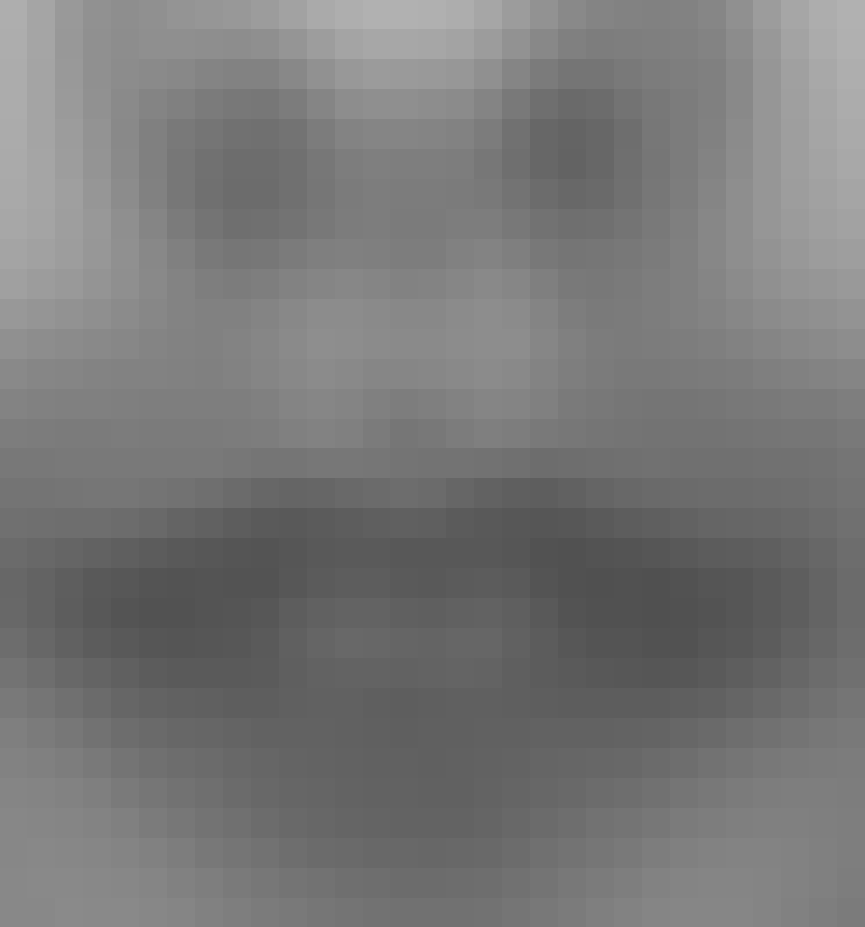
\includegraphics{figures/mouth_15.pdf}
\caption{Mean patch for mouth center top lip with `patch\_size = 15'}
\end{figure}

\hypertarget{patch-search-pred}{\subsection{Predicting a Facial Keypoint
using a Patch}\label{patch-search-pred}}

Having computed the mean patch for a particular keypoint, we can start
with predictons. For the predictions we run through the images and
search for the best match of the mean patch. As it would be very
inefficient and expensive to compare the match to all possible patch
positions, the Patch Search Learner only searches around the mean
keypoint positions of the training dataset. The size of the area around
this mean keypoint, where the learner searches, is determined by the
hyperparameter \texttt{search\_size}. Similar to the identification of
the outer coordinates of the patch, the search area is determined by
setting its center to the mean position and the width and height to
\texttt{2\ *\ search\_size\ +\ 1}. Afterwards the algorithm runs through
every pixel in the search area and the mean patch's center is set to the
pixel in order to calculate the match. The position in the search area
with the best match is used as prediction.

Again we are using the \texttt{mlR} interface to provide the
functionality. Therefore, we define the following function to make the
prediction part of the learner available to \texttt{mlR}. Before handing
over the data to our custom function, we extract the hyperparameters of
the current model and to be sure they have some value set them to the
default values in case they are \texttt{NULL}.

\begin{Shaded}
\begin{Highlighting}[]
\NormalTok{predictLearner.regr.patchSearch =}\StringTok{ }\NormalTok{function(.learner, .model, .newdata, ...) \{}
  \NormalTok{.patch_size =}\StringTok{ }\NormalTok{.model$learner$par.vals$patch_size}
  \NormalTok{.search_size =}\StringTok{ }\NormalTok{.model$learner$par.vals$search_size}

  \NormalTok{.patch_size =}\StringTok{ }\KeywordTok{ifelse}\NormalTok{(}\KeywordTok{is.null}\NormalTok{(.patch_size), }\DecValTok{10}\NormalTok{, .patch_size)}
  \NormalTok{.search_size =}\StringTok{ }\KeywordTok{ifelse}\NormalTok{(}\KeywordTok{is.null}\NormalTok{(.search_size), }\DecValTok{2}\NormalTok{, .search_size)}

  \KeywordTok{patchSearch.predict}\NormalTok{(.model,}
                      \DataTypeTok{f =} \KeywordTok{getTaskFormula}\NormalTok{(.model$task.desc),}
                      \DataTypeTok{d.te =} \NormalTok{.newdata,}
                      \DataTypeTok{patch_size =} \NormalTok{.patch_size,}
                      \DataTypeTok{search_size =} \NormalTok{.search_size,}
                      \NormalTok{...)}
\NormalTok{\}}
\end{Highlighting}
\end{Shaded}

Our custom function accepts the model, the formula, test data and the
hyperparameters as parameters. First, the mean patch is extracted from
the model and the target variable name is read from the formula.

\begin{Shaded}
\begin{Highlighting}[]
\NormalTok{patchSearch.predict <-}\StringTok{ }\NormalTok{function(model, f, d.te, }\DataTypeTok{patch_size =} \DecValTok{10}\NormalTok{, }\DataTypeTok{search_size =} \DecValTok{2}\NormalTok{)  \{}
  \NormalTok{mean.patch =}\StringTok{ }\NormalTok{model$learner.model}

  \CommentTok{# the coordinates we want to predict}
  \NormalTok{coord =}\StringTok{ }\KeywordTok{all.vars}\NormalTok{(f)[}\DecValTok{1}\NormalTok{]}
  \NormalTok{coord_x <-}\StringTok{ }\KeywordTok{paste}\NormalTok{(coord, }\StringTok{"x"}\NormalTok{, }\DataTypeTok{sep=}\StringTok{"_"}\NormalTok{)}
  \NormalTok{coord_y <-}\StringTok{ }\KeywordTok{paste}\NormalTok{(coord, }\StringTok{"y"}\NormalTok{, }\DataTypeTok{sep=}\StringTok{"_"}\NormalTok{)}
\end{Highlighting}
\end{Shaded}

Now the mean of the x and y coordinate is calculated based on the
training data. By using the hyperparameter \texttt{search\_size} we can
calculate the search area. As the mean positions of a keypoint could lie
so close to the border, that the patch would not lie completely inside
the image, we have to cut the search area by these pixels. The variable
\texttt{params} then contains all coordinates in the search area.

\begin{Shaded}
\begin{Highlighting}[]
  \CommentTok{# the average of them in the training set (our starting point)}
  \NormalTok{mean_x  <-}\StringTok{ }\KeywordTok{mean}\NormalTok{(d.train[, coord_x], }\DataTypeTok{na.rm=}\NormalTok{T)}
  \NormalTok{mean_y  <-}\StringTok{ }\KeywordTok{mean}\NormalTok{(d.train[, coord_y], }\DataTypeTok{na.rm=}\NormalTok{T)}

  \CommentTok{# search space: 'search_size' pixels centered on the average coordinates}
  \NormalTok{x1 <-}\StringTok{ }\KeywordTok{as.integer}\NormalTok{(mean_x)-search_size}
  \NormalTok{x2 <-}\StringTok{ }\KeywordTok{as.integer}\NormalTok{(mean_x)+search_size}
  \NormalTok{y1 <-}\StringTok{ }\KeywordTok{as.integer}\NormalTok{(mean_y)-search_size}
  \NormalTok{y2 <-}\StringTok{ }\KeywordTok{as.integer}\NormalTok{(mean_y)+search_size}

  \CommentTok{# ensure we only consider patches completely inside the image}
  \NormalTok{x1 <-}\StringTok{ }\KeywordTok{ifelse}\NormalTok{(x1-patch_size<}\DecValTok{1}\NormalTok{,  patch_size}\DecValTok{+1}\NormalTok{,  x1)}
  \NormalTok{y1 <-}\StringTok{ }\KeywordTok{ifelse}\NormalTok{(y1-patch_size<}\DecValTok{1}\NormalTok{,  patch_size}\DecValTok{+1}\NormalTok{,  y1)}
  \NormalTok{x2 <-}\StringTok{ }\KeywordTok{ifelse}\NormalTok{(x2+patch_size>}\DecValTok{96}\NormalTok{, }\DecValTok{96}\NormalTok{-patch_size, x2)}
  \NormalTok{y2 <-}\StringTok{ }\KeywordTok{ifelse}\NormalTok{(y2+patch_size>}\DecValTok{96}\NormalTok{, }\DecValTok{96}\NormalTok{-patch_size, y2)}

  \CommentTok{# build a list of all positions to be tested}
  \NormalTok{params <-}\StringTok{ }\KeywordTok{expand.grid}\NormalTok{(}\DataTypeTok{x =} \NormalTok{x1:x2, }\DataTypeTok{y =} \NormalTok{y1:y2)}
\end{Highlighting}
\end{Shaded}

We can now run through all test images and search for the best match of
the models mean patch in the search area. The outer loop is responsible
for running through the images, whereas the inner loop runs through all
coordinate combinations in the search area. For each coordinate
combination the patch with the same size as the models mean patch is
extracted. Both, the extracted patch and the mean patch are then
converted to a vector and the match between them is calculated by the
correlation amongst them. Afterwards, the coordinates and the
correlation is stored in a data frame, such that we can easily extract
the coordinates with the highest correlation value. The final step is to
retransform the two coordinates back to a single value to make them
compatible with the general data format we agreed upon. Thus, we have
our prediction.

\begin{Shaded}
\begin{Highlighting}[]
  \CommentTok{# for each image...}
  \NormalTok{r <-}\StringTok{ }\KeywordTok{foreach}\NormalTok{(}\DataTypeTok{i =} \DecValTok{1}\NormalTok{:}\KeywordTok{nrow}\NormalTok{(d.te), }\DataTypeTok{.combine=}\NormalTok{rbind) %do%}\StringTok{ }\NormalTok{\{}
    \NormalTok{im <-}\StringTok{ }\KeywordTok{matrix}\NormalTok{(}\DataTypeTok{data =} \NormalTok{d.te[i, }\StringTok{"Image"}\NormalTok{], }\DataTypeTok{nrow=}\DecValTok{96}\NormalTok{, }\DataTypeTok{ncol=}\DecValTok{96}\NormalTok{)}
    \NormalTok{if ((i %%}\StringTok{ }\DecValTok{100}\NormalTok{)==}\DecValTok{0}\NormalTok{) \{ }\KeywordTok{cat}\NormalTok{(}\KeywordTok{sprintf}\NormalTok{(}\StringTok{"Predicting %s for test image %d/%d}\CharTok{\textbackslash{}n}\StringTok{"}\NormalTok{, }
                                     \NormalTok{coord, i, }\KeywordTok{nrow}\NormalTok{(d.te))) \}}

    \CommentTok{# ... compute a score for each position ...}
    \NormalTok{r  <-}\StringTok{ }\KeywordTok{foreach}\NormalTok{(}\DataTypeTok{j =} \DecValTok{1}\NormalTok{:}\KeywordTok{nrow}\NormalTok{(params), }\DataTypeTok{.combine=}\NormalTok{rbind) %do%}\StringTok{ }\NormalTok{\{}
      \NormalTok{x     <-}\StringTok{ }\NormalTok{params$x[j]}
      \NormalTok{y     <-}\StringTok{ }\NormalTok{params$y[j]}
      \NormalTok{p     <-}\StringTok{ }\NormalTok{im[(x-patch_size):(x+patch_size), (y-patch_size):(y+patch_size)]}
      \NormalTok{score <-}\StringTok{ }\KeywordTok{cor}\NormalTok{(}\KeywordTok{as.vector}\NormalTok{(p), }\KeywordTok{as.vector}\NormalTok{(mean.patch))}
      \NormalTok{score <-}\StringTok{ }\KeywordTok{ifelse}\NormalTok{(}\KeywordTok{is.na}\NormalTok{(score), }\DecValTok{0}\NormalTok{, score)}
      \KeywordTok{data.frame}\NormalTok{(x, y, score)}
    \NormalTok{\}}

    \CommentTok{# ... and return the best}
    \NormalTok{best <-}\StringTok{ }\NormalTok{r[}\KeywordTok{which.max}\NormalTok{(r$score), }\KeywordTok{c}\NormalTok{(}\StringTok{"x"}\NormalTok{, }\StringTok{"y"}\NormalTok{)]}
    \NormalTok{best}
  \NormalTok{\}}

  \CommentTok{# retransform to single value}
  \NormalTok{result <-}\StringTok{ }\NormalTok{(}\KeywordTok{round}\NormalTok{(r[}\DecValTok{1}\NormalTok{]) -}\StringTok{ }\DecValTok{1}\NormalTok{) *}\StringTok{ }\DecValTok{96} \NormalTok{+}\StringTok{ }\KeywordTok{round}\NormalTok{(r[}\DecValTok{2}\NormalTok{])}
  \NormalTok{result[}\DecValTok{1}\NormalTok{]$x}
\ErrorTok{\}}
\end{Highlighting}
\end{Shaded}

\hypertarget{deep-neural-nets}{\section{Tensorflow in Combination With
R}\label{deep-neural-nets}}

Tensorflow (TF) is an open source library for machine learning,
originally developed by Google. It became extremely popular recently,
with about 42,500 stars and 20,000 forks on Github.

The main principle behind TF are so called \emph{computational data flow
graphs}. A machine learning model (like e.g.~a neural network) is
described in its enirety through such a graph. All nodes in that graph
are placeholder objects. Only after the whole graph has been
initialized, actual data is fed into the nodes. This makes it easier to
quickly change the structure of the model, without having to worry about
keeping the model with all weights etc. in memory.

Initially, Google provided an API for Python and C++, but the team
behind RStudio recently released a
\href{https://github.com/rstudio/tensorflow}{package}, that provides a
TF Interface for R. Although the project is still in a quite early
stage, we decided to work with this package in order to get a flexible
library for deep learning projects - which are surprisingly rare in R.
We were eager to be part of the very early adopters of the R/Tensorflow
combination, so that we even submitted some
\href{https://github.com/rstudio/tensorflow/issues/37}{error fixes} on
Github in order to get the package to work on our system.

\subsection{Deep Neural Nets for Facial Keypoints
Detection}\label{deep-neural-nets-for-facial-keypoints-detection}

Since we want to predict 15 keypoints in the face of a person, each
having an x- and a y-coordinate, the prediciton of the statistical model
has to provide 30 values. Moreover, the facial keypoints detection
problem is a regression problem: the predicted number for a certain
keypoint position contains spatial information, which would be lost if
the prediction would be treated as a classification problem (i.e.~no
numerical order of the values). As the analyzed data set's images have
the dimensions {[}96, 96{]}, the predicted values should also lie in
that range.

The nature of multi-node layers in neural networks makes it easy to
obtain multiple outputs (as compared to other model-types where it might
be necessary to create one model for every prediction value). In
addition, especially convolutional neural networks have proven to work
very well in image related problems (and more generally in problems
where spatial information matters). We have built and successfully
trained a multi-layer perceptron and a convolutional neural network,
which will be described in the following.

\subsection{Multi-Layer Perceptron
(MLP)}\label{multi-layer-perceptron-mlp}

\subsubsection{Data Preparation}\label{data-preparation}

After loading the tensorflow package

\begin{Shaded}
\begin{Highlighting}[]
\KeywordTok{library}\NormalTok{(tensorflow)}
\end{Highlighting}
\end{Shaded}

the data has to be prepared in order for TF to process it. First, the
data has to be in the matrix data format.

\begin{Shaded}
\begin{Highlighting}[]
\NormalTok{train.x =}\StringTok{ }\KeywordTok{as.matrix}\NormalTok{(d.train$Image)}
\NormalTok{train.y =}\StringTok{ }\KeywordTok{as.matrix}\NormalTok{(d.train[,-}\DecValTok{31}\NormalTok{])}
\end{Highlighting}
\end{Shaded}

TF expects input to be scaled to values in the interval {[}0, 1{]}, so
we scale the pixel intensities (i.e.~feature values) by dividing by 255
(where 0 is a black pixel and 255 is a white pixel).

\begin{Shaded}
\begin{Highlighting}[]
\NormalTok{train.x =}\StringTok{ }\NormalTok{train.x /}\StringTok{ }\DecValTok{255}
\end{Highlighting}
\end{Shaded}

On the middle of the image, we place the origin of the coordinate
system, such that the left (/down) most point is -1 and the right (/up)
most point is +1. Each of the target values is scaled into this {[}-1,
1{]} interval (from prior {[}0, 96{]}).

\begin{Shaded}
\begin{Highlighting}[]
\NormalTok{train.y =}\StringTok{ }\NormalTok{(train.y -}\StringTok{ }\DecValTok{48}\NormalTok{) /}\StringTok{ }\DecValTok{48}
\end{Highlighting}
\end{Shaded}

\subsubsection{Hyperparameters}\label{hyperparameters}

We control four different hyperparameters, that can be adapted once we
decided for a certain network structure:

\begin{itemize}
\tightlist
\item
  Learning Rate. Controls how big of a step the optimization algorithm
  should take in every training step. High values mean potentially
  faster results from training, but might miss out on optima, by
  ``overstepping'' them.
\item
  Number of training epochs. One epoch marks one run-through of all
  training data through the training process.
\item
  Batch size. From the training data, a random batch is drawn on every
  training step. Only this data is then used to further train the
  network. After one training epoch, all batches in the training set
  have been used.
\item
  Display Step. How often we want to log the current status.
\end{itemize}

\begin{Shaded}
\begin{Highlighting}[]
\NormalTok{learning_rate =}\StringTok{ }\FloatTok{0.001}
\NormalTok{training_epochs =}\StringTok{ }\NormalTok{1000L}
\NormalTok{batch_size =}\StringTok{ }\NormalTok{50L}
\NormalTok{display_step =}\StringTok{ }\NormalTok{1L}
\end{Highlighting}
\end{Shaded}

\subsubsection{Network Structure}\label{network-structure}

We experimented with different depths of the network but realized
quickly that training on a CPU (as opposed to a GPU) puts certain limits
on the complexity. Nevertheless, we achieved decent results with the
following structure (in combination with the above hyperparameters).

\begin{Shaded}
\begin{Highlighting}[]
\NormalTok{n_input =}\StringTok{ }\NormalTok{9216L }\CommentTok{# 96x96 pixels}
\NormalTok{n_hidden_1 =}\StringTok{ }\NormalTok{256L }\CommentTok{# 1st layer number of features}
\NormalTok{n_hidden_2 =}\StringTok{ }\NormalTok{256L }\CommentTok{# 2nd layer number of features}
\NormalTok{n_classes =}\StringTok{ }\NormalTok{30L }\CommentTok{# 15 x, 15 y coordinates}
\end{Highlighting}
\end{Shaded}

\subsubsection{Tensorflow Graph}\label{tensorflow-graph}

First we create some placeholder variables to hold the input (x) and the
output (y).

\begin{Shaded}
\begin{Highlighting}[]
\NormalTok{x =}\StringTok{ }\NormalTok{tf$}\KeywordTok{placeholder}\NormalTok{(tf$float32, }\KeywordTok{shape}\NormalTok{(}\OtherTok{NULL}\NormalTok{, n_input))}
\NormalTok{y =}\StringTok{ }\NormalTok{tf$}\KeywordTok{placeholder}\NormalTok{(tf$float32, }\KeywordTok{shape}\NormalTok{(}\OtherTok{NULL}\NormalTok{, n_classes))}
\end{Highlighting}
\end{Shaded}

Then we create two convenience functions to simplify the creation of
weight and bias variables. These variables get initialized with a random
number, whose extent can be modified via the \emph{stddev} parameter.

\begin{Shaded}
\begin{Highlighting}[]
\NormalTok{weight_variable <-}\StringTok{ }\NormalTok{function(shape) \{}
  \NormalTok{initial <-}\StringTok{ }\NormalTok{tf$}\KeywordTok{truncated_normal}\NormalTok{(shape, }\DataTypeTok{stddev=}\FloatTok{0.1}\NormalTok{)}
  \NormalTok{tf$}\KeywordTok{Variable}\NormalTok{(initial)}
\NormalTok{\}}

\NormalTok{bias_variable <-}\StringTok{ }\NormalTok{function(shape) \{}
  \NormalTok{initial <-}\StringTok{ }\NormalTok{tf$}\KeywordTok{constant}\NormalTok{(}\FloatTok{0.1}\NormalTok{, }\DataTypeTok{shape=}\NormalTok{shape)}
  \NormalTok{tf$}\KeywordTok{Variable}\NormalTok{(initial)}
\NormalTok{\}}
\end{Highlighting}
\end{Shaded}

Afterwards we define the actual model in the graph. (Hidden) Layer 1 is
a matrix multiplication of the input x. The shape is defined by the
parameters specified in the \textbf{Network Structure} section. The
output of this layer runs through the \emph{ReLU} (\emph{Rectified
Linear Unit}) activation function \(f(x)=max(0, x)\), which sets all
negative output to 0. The output is fed into the second (hidden) layer,
which performs another matrix multiplication and has the previosuly
defined shape. The activation function is again a ReLU. Finally, the
output is fed into the output layer, which has exactly 30 nodes to
represent all 15 coordinate pairs of the facial keypoints.

\begin{Shaded}
\begin{Highlighting}[]
\NormalTok{layer1 =}\StringTok{ }\NormalTok{tf$}\KeywordTok{add}\NormalTok{(tf$}\KeywordTok{matmul}\NormalTok{(x, }\KeywordTok{weight_variable}\NormalTok{(}\KeywordTok{shape}\NormalTok{(n_input, n_hidden_1))),}
                \KeywordTok{bias_variable}\NormalTok{(}\KeywordTok{shape}\NormalTok{(n_hidden_1)))}
\NormalTok{layer1 =}\StringTok{ }\NormalTok{tf$nn$}\KeywordTok{relu}\NormalTok{(layer1)}

\NormalTok{layer2 =}\StringTok{ }\NormalTok{tf$}\KeywordTok{add}\NormalTok{(tf$}\KeywordTok{matmul}\NormalTok{(layer1, }\KeywordTok{weight_variable}\NormalTok{(}\KeywordTok{shape}\NormalTok{(n_hidden_1, n_hidden_2))),}
                \KeywordTok{bias_variable}\NormalTok{(}\KeywordTok{shape}\NormalTok{(n_hidden_2)))}
\NormalTok{layer2 =}\StringTok{ }\NormalTok{tf$nn$}\KeywordTok{relu}\NormalTok{(layer2)}

\NormalTok{out_layer =}\StringTok{ }\NormalTok{tf$}\KeywordTok{matmul}\NormalTok{(layer2, }\KeywordTok{weight_variable}\NormalTok{(}\KeywordTok{shape}\NormalTok{(n_hidden_2, n_classes))) +}
\StringTok{            }\KeywordTok{bias_variable}\NormalTok{(}\KeywordTok{shape}\NormalTok{(n_classes))}
\end{Highlighting}
\end{Shaded}

Now we define the cost function of the optimization method, which is the
MSE. For the optimization method itself we used the popular Adam
Optimizer, which usually
\href{https://arxiv.org/pdf/1412.6980v8.pdf}{converges faster} than many
other optimizers such as stochastic gradient decent. The accuracy
measure used in the Kaggle competition is the RMSE. Therefore we can get
an estimate of our performance on test data by taking the square root of
the MSE. We multiply by 48 in order to account for the previous scaling
of the training target data.

\begin{Shaded}
\begin{Highlighting}[]
\NormalTok{cost =}\StringTok{ }\NormalTok{tf$}\KeywordTok{reduce_mean}\NormalTok{(tf$}\KeywordTok{square}\NormalTok{(out_layer -}\StringTok{ }\NormalTok{y))}
\NormalTok{optimizer =}\StringTok{ }\NormalTok{tf$train$}\KeywordTok{AdamOptimizer}\NormalTok{(}\DataTypeTok{learning_rate =} \NormalTok{learning_rate)$}\KeywordTok{minimize}\NormalTok{(cost)}
\NormalTok{accuracy =}\StringTok{ }\NormalTok{tf$}\KeywordTok{sqrt}\NormalTok{(cost) *}\StringTok{ }\DecValTok{48}
\end{Highlighting}
\end{Shaded}

Finally, this graph definition can not be interfaced until a TF session
is launched and the TF variables we just created are initialized.

\begin{Shaded}
\begin{Highlighting}[]
\NormalTok{sess <-}\StringTok{ }\NormalTok{tf$}\KeywordTok{Session}\NormalTok{()}
\NormalTok{sess$}\KeywordTok{run}\NormalTok{(tf$}\KeywordTok{initialize_all_variables}\NormalTok{())}
\end{Highlighting}
\end{Shaded}

\subsubsection{Training and Evaluating the
Model}\label{training-and-evaluating-the-model}

First we define a function that makes it easy to pass batches into the
training mechanism.

\begin{Shaded}
\begin{Highlighting}[]
\NormalTok{nextBatchIndices <-}\StringTok{ }\NormalTok{function(indices, batchNr, batch_size) \{}
  \NormalTok{position =}\StringTok{ }\NormalTok{batchNr *}\StringTok{ }\NormalTok{batch_size -}\StringTok{ }\NormalTok{batch_size +}\StringTok{ }\DecValTok{1}
  \NormalTok{if ((position +}\StringTok{ }\NormalTok{batch_size) >}\StringTok{ }\KeywordTok{length}\NormalTok{(indices)) \{}
    \KeywordTok{return}\NormalTok{(indices[position:}\KeywordTok{length}\NormalTok{(indices)])}
  \NormalTok{\}}
  \KeywordTok{return}\NormalTok{(indices[position:(position +}\StringTok{ }\NormalTok{batch_size -}\StringTok{ }\DecValTok{1}\NormalTok{)])}
\NormalTok{\}}
\end{Highlighting}
\end{Shaded}

The number of batches for the training set is indirectly given by the
hyperparameter \emph{batch\_size}.

\begin{Shaded}
\begin{Highlighting}[]
\NormalTok{numberOfBatches =}\StringTok{ }\KeywordTok{ceiling}\NormalTok{(}\KeywordTok{nrow}\NormalTok{(train.x) /}\StringTok{ }\NormalTok{batch_size)}
\end{Highlighting}
\end{Shaded}

The training process takes place in two nested loops. The outer loop
simply cycles for the specified number of training epochs, every time
shuffling the indices of the training set in order to provide ``fresh''
batches for training, which helps regularizing (reduce overfitting) the
network. In the inner loop the previosuly defined function is used to
get the next batch of data, which is then used for training. In addition
the current status of the progress is printed to the terminal.

\begin{Shaded}
\begin{Highlighting}[]
\NormalTok{for(epoch in }\KeywordTok{seq_len}\NormalTok{(training_epochs)) \{}
  \NormalTok{shuffledIndices =}\StringTok{ }\KeywordTok{sample}\NormalTok{(}\KeywordTok{seq_len}\NormalTok{(}\KeywordTok{nrow}\NormalTok{(train.x)))}

  \NormalTok{for(batchNr in }\KeywordTok{seq_len}\NormalTok{(numberOfBatches)) \{}
    \NormalTok{rowIndices =}\StringTok{ }\KeywordTok{nextBatchIndices}\NormalTok{(shuffledIndices, batchNr, batch_size)}

    \NormalTok{train_accuracy <-}\StringTok{ }\NormalTok{sess$}\KeywordTok{run}\NormalTok{(accuracy, }\DataTypeTok{feed_dict =} \KeywordTok{dict}\NormalTok{(}\DataTypeTok{x =} \NormalTok{train.x[rowIndices, ], }
                                                          \DataTypeTok{y =} \NormalTok{train.y[rowIndices, ]))}
    \KeywordTok{cat}\NormalTok{(}\KeywordTok{sprintf}\NormalTok{(}\StringTok{"Epoch: %d | Batch: %d/%d | Training RMSE: %g}\CharTok{\textbackslash{}n}\StringTok{"}\NormalTok{, }
                \NormalTok{epoch, batchNr, numberOfBatches, train_accuracy))}

    \NormalTok{sess$}\KeywordTok{run}\NormalTok{(optimizer, }\DataTypeTok{feed_dict =} \KeywordTok{dict}\NormalTok{(}\DataTypeTok{x =} \NormalTok{train.x[rowIndices, ], }
                                         \DataTypeTok{y =} \NormalTok{train.y[rowIndices, ]))}
  \NormalTok{\}}
\NormalTok{\}}
\end{Highlighting}
\end{Shaded}

After training is completed, one could assess the estimated performance
on test data. This is not really necessary, as Kaggle provides us with a
concrete accuracy score. However, using suffienctly large batch sizes
can yield reasonable performance estimations just using the current
batch already during training (like we do in the code above). Due to the
shuffling + use of multiple epochs (emulates \emph{replacement}) this is
very similar to the bootstrap approach. For quick evaluations, one could
also just split the training set into \emph{train} and \emph{test} and
then feed the test data into the TF model.

\begin{Shaded}
\begin{Highlighting}[]
\NormalTok{test_accuracy <-}\StringTok{ }\NormalTok{sess$}\KeywordTok{run}\NormalTok{(accuracy, }\DataTypeTok{feed_dict =} \KeywordTok{dict}\NormalTok{(}\DataTypeTok{x =} \NormalTok{test.x, }\DataTypeTok{y =} \NormalTok{test.y))}
\KeywordTok{cat}\NormalTok{(}\KeywordTok{sprintf}\NormalTok{(}\StringTok{"Test RMSE: %g"}\NormalTok{, test_accuracy))}
\end{Highlighting}
\end{Shaded}

This test data can then be used to actually plot the output of the
neural net on one of the corresponding images. The multiplications serve
the purpose of rescaling.

\begin{Shaded}
\begin{Highlighting}[]
\NormalTok{data =}\StringTok{ }\NormalTok{test.x *}\StringTok{ }\DecValTok{255}
\NormalTok{pred =}\StringTok{ }\NormalTok{sess$}\KeywordTok{run}\NormalTok{(out_layer, }\DataTypeTok{feed_dict =} \KeywordTok{dict}\NormalTok{(}\DataTypeTok{x =} \NormalTok{test.x)) *}\StringTok{ }\DecValTok{48} \NormalTok{+}\StringTok{ }\DecValTok{48}
\NormalTok{fkdR::}\KeywordTok{plotFacialKeypoints}\NormalTok{(data, }\DecValTok{1}\NormalTok{, pred)}
\end{Highlighting}
\end{Shaded}

\subsubsection{Submission File}\label{submission-file}

Using the fkdR package, creating a submission file for the Kaggle
competition only takes three simple steps. First, the test data set has
to be scaled in order to be processed by our TF model. Second, the model
has to predict the target value by feeding it the test data and scaling
it back to the original scale. Third, the \emph{writeSubmissionFile}
function has to be called.

\begin{Shaded}
\begin{Highlighting}[]
\NormalTok{data =}\StringTok{ }\NormalTok{d.test$Image /}\StringTok{ }\DecValTok{255}
\NormalTok{pred =}\StringTok{ }\NormalTok{sess$}\KeywordTok{run}\NormalTok{(out_layer, }\DataTypeTok{feed_dict =} \KeywordTok{dict}\NormalTok{(}\DataTypeTok{x =} \NormalTok{data)) *}\StringTok{ }\DecValTok{48} \NormalTok{+}\StringTok{ }\DecValTok{48}
\NormalTok{fkdR::}\KeywordTok{writeSubmissionFile}\NormalTok{(}\DataTypeTok{predictions =} \NormalTok{pred, }\StringTok{"/path/for/submissions/"}\NormalTok{)}
\end{Highlighting}
\end{Shaded}

\subsubsection{Save and Restore}\label{save-and-restore}

Finally, we made an effort to save and restore the TF model (including
the trained weights and biases), so that there is no data loss after
restarting the R session.

\begin{Shaded}
\begin{Highlighting}[]
\CommentTok{# Save data}
\NormalTok{saver <-}\StringTok{ }\NormalTok{tf$train$}\KeywordTok{Saver}\NormalTok{()}
\NormalTok{data_file <-}\StringTok{ }\NormalTok{saver$}\KeywordTok{save}\NormalTok{(sess, }\KeywordTok{paste0}\NormalTok{(}\StringTok{"/path/for/submissions/"}\NormalTok{, }
                                     \StringTok{"fkdr_mlp_1000epochs.ckpt"}\NormalTok{))}

\CommentTok{# Restore Data}
\NormalTok{sess =}\StringTok{ }\NormalTok{tf$}\KeywordTok{Session}\NormalTok{()}
\NormalTok{restorer =}\StringTok{ }\NormalTok{tf$train$}\KeywordTok{import_meta_graph}\NormalTok{(}\KeywordTok{paste0}\NormalTok{(}\StringTok{"/path/for/submissions/"}\NormalTok{, }
                                             \StringTok{"fkdr_mlp_1000epochs.ckpt.meta"}\NormalTok{))}

\NormalTok{restorer$}\KeywordTok{restore}\NormalTok{(sess, tf$train$}\KeywordTok{latest_checkpoint}\NormalTok{(}\StringTok{"/path/for/submissions/"}\NormalTok{))}
\end{Highlighting}
\end{Shaded}

Unfortunately, this (as of now) leads to unexpected behavior, although
the code should be correct. We filed a Github issue for this and are in
a conversation with two of the lead RStudio/Tensorflow programmers.

\subsection{Convolutional Neural Network
(CNN)}\label{convolutional-neural-network-cnn}

In order to build a convolutional neural network, we need two more
convenience functions and of course a different layer structure.

\subsubsection{Convolution, Max Pooling, Dropout and Fully Connected
Layer}\label{convolution-max-pooling-dropout-and-fully-connected-layer}

In the following, the process of convolution and pooling will be
described in general, followed by the code that implements the
theoretical excursion.

\paragraph{Theory}\label{theory}

\subparagraph{Convolution}\label{convolution}

A convolutional layer is essentially a set of so called filters, which
can be trained. In contrast to traditional image recognition techniques,
where filters like the \emph{Sobel Edge Detector} might be used to
detect certain features in an image, the filters in the convolutional
layer are randomly initialized (not predefined) and they are solely
shaped through training the network.

A filter is essentially a window (typically 5 by 5 pixels) that slides
(--\textgreater{} \textbf{convolves}) across an image. For colored
images, the window is a cube (5x5x\textbf{3}), since the image contains
three color channels.

Once a network is trained sufficiently, one of the filters might
actually look like an edge (similar to Sobel for instance). The
following picture shows an exemplary set of learned filters that can
detect edges and other important features in images.

\begin{figure}
\centering
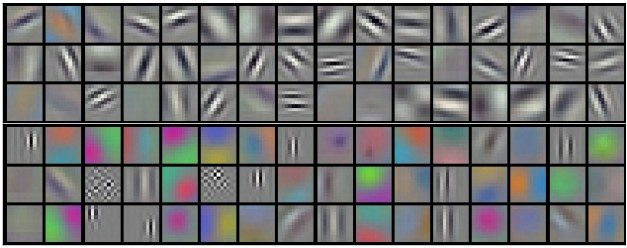
\includegraphics{figures/learned_filters_example.jpeg}
\caption{Example of learned filters (Krizhevsky et al. 2014)}
\end{figure}

When using the trained network to make a prediction, the filter window
slides across the image. Every pixel in the filter window gets matched
with the underlying part of the image. If the pixels are similar, this
contributes to a high activation of the filter. For the edge filter,
this means that there is an edge in the image that looks similar to the
edge that the filter represents.

It is common to pad the image with zeros around the edges in order for
the convolution operation not to alter the spatial dimensions of the
input.

\subparagraph{Max Pooling}\label{max-pooling}

Max Pooling is a way to reduce the size of the feature map. Again, we
slide a window (typically 2x2 pixels) across the image/activation map
and produce a new, smaller map (when using 2x2 pixels: one quarter of
the size). This is done by simply taking the highest value inside the
sliding window as the only pixel for the new map. This causes the most
prominent features of the map to persist, while less relevant
information goes away. This has two benefits: it reduces computational
cost, as less parameters have to be trained for the individual image
maps and it helps to reduce overfitting, as the information gets more
abstract.

\subparagraph{Dropout}\label{dropout}

Dropout is another regularization technique, that works very well for
\href{http://neuralnetworksanddeeplearning.com/chap3.html}{various
reasons}. Essentially, it forces the neural net to learn multiple
independent representations of the same data by alternately randomly
disabling neurons in the learning phase.

\subparagraph{Fully Connected Layer}\label{fully-connected-layer}

The last (several) layer(s) of a convolutional net is a fully connected
layer. Already known from the Multi-Layer Perceptron, it connects all
nodes (30 in the current case) with all nodes from the previous layer.

The following image compares an abstract representation of a MLP vs.~a
CNN. The right side shows how the pooling operation reshapes the volume
of activation maps, as the images get smaller and smaller. A fully
connected layer as seen on the left side is also added in a CNN as the
very last step.

\begin{figure}
\centering
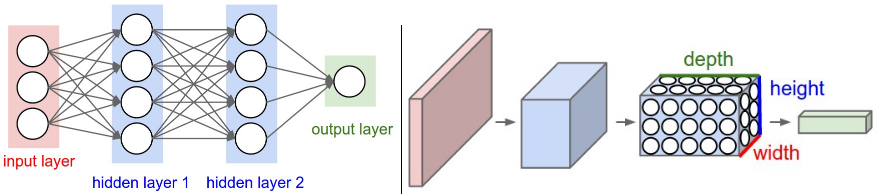
\includegraphics{figures/mlp_vs_cnn.png}
\caption{Andrej Karpathy,
\url{http://cs231n.github.io/convolutional-networks/} retreived on 7 Jan
2017}
\end{figure}

\paragraph{Practice}\label{practice}

\subparagraph{Convenience Functions}\label{convenience-functions}

In addition to the \emph{weight\_variable} and \emph{bias\_variable}
functions, we create functions to handle convolution and max pooling.
The stride (how many pixels does the window move per step) is set to 1
for convolution, and we use 2x2 max pooling.

\begin{Shaded}
\begin{Highlighting}[]
\NormalTok{conv2d <-}\StringTok{ }\NormalTok{function(x, W) \{}
  \NormalTok{tf$nn$}\KeywordTok{conv2d}\NormalTok{(x, W, }\DataTypeTok{strides=}\KeywordTok{c}\NormalTok{(1L, 1L, 1L, 1L), }\DataTypeTok{padding=}\StringTok{'SAME'}\NormalTok{)}
\NormalTok{\}}

\NormalTok{max_pool_2x2 <-}\StringTok{ }\NormalTok{function(x) \{}
  \NormalTok{tf$nn$}\KeywordTok{max_pool}\NormalTok{(}
    \NormalTok{x,}
    \DataTypeTok{ksize=}\KeywordTok{c}\NormalTok{(1L, 2L, 2L, 1L),}
    \DataTypeTok{strides=}\KeywordTok{c}\NormalTok{(1L, 2L, 2L, 1L),}
    \DataTypeTok{padding=}\StringTok{'SAME'}\NormalTok{)}
\NormalTok{\}}
\end{Highlighting}
\end{Shaded}

\subparagraph{Tensorflow Graph
Definition}\label{tensorflow-graph-definition}

We stack several of the layer types described in the \textbf{Theory}
section on top of each other in an alternating format.

\begin{enumerate}
\def\labelenumi{\arabic{enumi})}
\tightlist
\item
  Convolutional layer with 32 filters and a 5x5 window size.
\end{enumerate}

\begin{itemize}
\tightlist
\item
  Image data needs to have four-dimensional shape for internal reasons.
\item
  Activation function is ReLU.
\end{itemize}

\begin{enumerate}
\def\labelenumi{\arabic{enumi})}
\setcounter{enumi}{1}
\tightlist
\item
  Max Pooling with 2x2 window.
\item
  Convolutional layer with 64 filters and a 5x5 window size.
\item
  Max Pooling with 2x2 window.
\item
  Fully connected layer with 1024 neurons to process on the entire
  image.
\end{enumerate}

\begin{itemize}
\tightlist
\item
  (Apply the dropout technique for regularization).
\end{itemize}

\begin{enumerate}
\def\labelenumi{\arabic{enumi})}
\setcounter{enumi}{5}
\tightlist
\item
  Fully connected layer with 30 output neurons.
\end{enumerate}

\begin{Shaded}
\begin{Highlighting}[]
\NormalTok{## First layer (convolution)}
\NormalTok{W_conv1 <-}\StringTok{ }\KeywordTok{weight_variable}\NormalTok{(}\KeywordTok{shape}\NormalTok{(5L, 5L, 1L, 32L))}
\NormalTok{b_conv1 <-}\StringTok{ }\KeywordTok{bias_variable}\NormalTok{(}\KeywordTok{shape}\NormalTok{(32L))}
\NormalTok{x_image <-}\StringTok{ }\NormalTok{tf$}\KeywordTok{reshape}\NormalTok{(x, }\KeywordTok{shape}\NormalTok{(-1L, 96L, 96L, 1L))}
\NormalTok{h_conv1 <-}\StringTok{ }\NormalTok{tf$nn$}\KeywordTok{relu}\NormalTok{(}\KeywordTok{conv2d}\NormalTok{(x_image, W_conv1) +}\StringTok{ }\NormalTok{b_conv1)}
\NormalTok{## Second layer (pooling)}
\NormalTok{h_pool1 <-}\StringTok{ }\KeywordTok{max_pool_2x2}\NormalTok{(h_conv1)}
\NormalTok{## Third layer (convolution)}
\NormalTok{W_conv2 <-}\StringTok{ }\KeywordTok{weight_variable}\NormalTok{(}\DataTypeTok{shape =} \KeywordTok{shape}\NormalTok{(5L, 5L, 32L, 64L))}
\NormalTok{b_conv2 <-}\StringTok{ }\KeywordTok{bias_variable}\NormalTok{(}\DataTypeTok{shape =} \KeywordTok{shape}\NormalTok{(64L))}
\NormalTok{h_conv2 <-}\StringTok{ }\NormalTok{tf$nn$}\KeywordTok{relu}\NormalTok{(}\KeywordTok{conv2d}\NormalTok{(h_pool1, W_conv2) +}\StringTok{ }\NormalTok{b_conv2)}
\NormalTok{## Fourth layer (pooling)}
\NormalTok{h_pool2 <-}\StringTok{ }\KeywordTok{max_pool_2x2}\NormalTok{(h_conv2)}
\NormalTok{## Fifth layer (fully connected)}
\NormalTok{W_fc1 <-}\StringTok{ }\KeywordTok{weight_variable}\NormalTok{(}\KeywordTok{shape}\NormalTok{(36864L, 1024L))}
\NormalTok{b_fc1 <-}\StringTok{ }\KeywordTok{bias_variable}\NormalTok{(}\KeywordTok{shape}\NormalTok{(1024L))}
\NormalTok{h_pool2_flat <-}\StringTok{ }\NormalTok{tf$}\KeywordTok{reshape}\NormalTok{(h_pool2, }\KeywordTok{shape}\NormalTok{(-1L, 24L *}\StringTok{ }\NormalTok{24L *}\StringTok{ }\NormalTok{64L))}
\NormalTok{h_fc1 <-}\StringTok{ }\NormalTok{tf$nn$}\KeywordTok{relu}\NormalTok{(tf$}\KeywordTok{matmul}\NormalTok{(h_pool2_flat, W_fc1) +}\StringTok{ }\NormalTok{b_fc1)}
\NormalTok{## Dropout}
\NormalTok{keep_prob <-}\StringTok{ }\NormalTok{tf$}\KeywordTok{placeholder}\NormalTok{(tf$float32)}
\NormalTok{h_fc1_drop <-}\StringTok{ }\NormalTok{tf$nn$}\KeywordTok{dropout}\NormalTok{(h_fc1, keep_prob)}
\NormalTok{## Sixth layer (readout, fully connected)}
\NormalTok{W_fc2 <-}\StringTok{ }\KeywordTok{weight_variable}\NormalTok{(}\KeywordTok{shape}\NormalTok{(1024L, 30L))}
\NormalTok{b_fc2 <-}\StringTok{ }\KeywordTok{bias_variable}\NormalTok{(}\KeywordTok{shape}\NormalTok{(30L))}
\NormalTok{y_conv <-}\StringTok{ }\NormalTok{tf$}\KeywordTok{matmul}\NormalTok{(h_fc1_drop, W_fc2) +}\StringTok{ }\NormalTok{b_fc2}
\end{Highlighting}
\end{Shaded}

Training and evaluating the network follows the same principle as our
MLP implementation.

\section{Discussion and Comparison}\label{discussion-and-comparison}

We made predictions based on three different methods. The first one was
the Patch Search Learner proposed by the authors of the Kaggle
competition. We tried to improve the results by tuning and resampling
and furthermore histogram equalized the images first to improve
contrast. We experienced Patch Search as a rather simple yet effective
and intuitive approach. It is easy to setup and once the hyperparameters
are tuned and the model is trained, it runs relatively fast. However, it
has some important limitations:

It works best, if all images are similarly aligned (i.e.~the face should
fill the image as much as possible) and the faces are horizontally
aligned (i.e.~both eyes are lying on one horizontal line). This leads to
the best mean patches, as it would otherwise become blured and more
difficult to be found in an image. The alignment is not only important
for the training of mean patches, but also for the predictions. If the
patch is horizontally aligned it would e.g.~not match a face, that is
turned by 90 degrees or smaller. Furthermore, during the definition of
the search area, pixels which are close to the borders are cut out, such
that keypoints at the border would not be able to detected. This is kind
of ironic, as if all images are similarly aligned, the detection of
positions of keypoints becomes rather trivial, as they are very close to
each other among all images. Moreover, the Patch Search Learner ignores
all interdependencies between keypoints, which could also yield some
worthy information for predictions. The dataset of the Kaggle contest
fortunately offered very similarly aligned images (it contained just
some outlier images, where the faces where rotated, scaled or more than
one face was in the image), such that the prediction accuracy was
already good.

The drawbacks of the Patch Search Learner motivated us to search for
methods which are better suited for more general images. These are the
Deep Neural Nets introduced in
\protect\hyperlink{deep-neural-nets}{section 4}. They are a lot more
robust against rotated and scaled images than the Patch Search Learner.
The MLP is the simplest form of deep learning, why it was a good
starting point into Deep Neural Nets. It typically has less parameters
than CNN and can therefore be faster trained. However, it has still some
limitations regarding suitability for images. I.e. images typically have
a lot of features that are not abstracted in a MLP, because it lacks
techniques like Max Pooling. Thus, it is not feasible for training with
large images. Moreover, spatial relationships of features are factored
in less than in CNNs. Anyway, for the Kaggle dataset it yielded already
better results than the Patch Search Learner.

As already indicated, the way to go for keypoint detection in images is
the construction of a CNN. Altouh deep inside a CNN is still a MLP just
with a special structure, it provides better results especially for
images, as it contains repetitive blocks of neurons that are applied
accross space (e.g.~for iamges) or time (e.g.~for audio signals).
Therefore, they work well for problems where the spatial relationship of
features matters. We could confirm this, as the CNNs yielded the best
results among all three methods.

\section{Conclusion and Outlook}\label{conclusion-and-outlook}

During the project we went from simple methods like the Patch Search
Learner to advanced methods like the Convolutional Neural Net. We
discovered the high potential of Deep Learning Algorithms and faced the
complexity of properly setting up such algorithms. Limitied computation
power as well as limited time unfortunately did not let us take
advantage of the full potential of them, which motivates us to give an
outlook on how to improve our results.

First, the input data can be improved in order to improve results.
Obiously more training data improves the models. This could with the
Kaggle dataset e.g.~be achieved by mirroring the images. We decided to
leave this for the outlook, to save computation time. For patch search
the results could further be improved by first cropping and rotating the
images, such that all of them are rather similarly aligned. For training
images this should be rather straightforward as we know the keypoints
and can guess the borders of the face by them. Doing this automatically
for test images could become complex, because it is another face
recognition step which has the same difficulties as finding the
keypoints themselves. Therefore using Deep Learning methods is more
promising, as it is more robust against rotations and scalings.

The MLP and CNN leave much room for improvements, as the composition of
layers can be changed. Tuning them is not trivial and a task, that needs
quite a lot of computation power. Furthermore, as of now, there is no
recommendation in research on how layers should be composed in order to
achieve best results. With more computation power, some tuning, more
training data and maybe a lot of try and error, especially the CNN could
still be heavily improved.


\end{document}
